\documentclass[11pt,a4paper]{article}
\usepackage[utf8]{inputenc}
\usepackage[T1]{fontenc}
\usepackage[french]{babel}
\usepackage{graphicx}
\usepackage{amsmath}
\usepackage{amssymb}
\usepackage{siunitx}
\usepackage{booktabs}
\usepackage{geometry}
\usepackage{caption}
\usepackage{subcaption}
\usepackage{hyperref}

\geometry{margin=2.5cm}

\title{Analyse statistique de l'émission de la source Am-241\\
\large Simulation Geant4 -- 100\,000 événements}
\author{Analyse des résultats de simulation}
\date{\today}

\begin{document}

\maketitle

\begin{abstract}
Ce document présente l'analyse statistique de l'émission de photons par une source d'américium-241 simulée avec Geant4. L'étude porte sur la distribution des gammas émis par événement, la répartition par raie caractéristique, le transport jusqu'à la cible d'eau, et les pertes dans l'air.
\end{abstract}

%==============================================================================
\section{Distribution du nombre de gammas par événement}
%==============================================================================

La figure~\ref{fig:gamma_per_event} présente la distribution du nombre de photons $\gamma$ émis par désintégration (événement).

\begin{figure}[htbp]
    \centering
    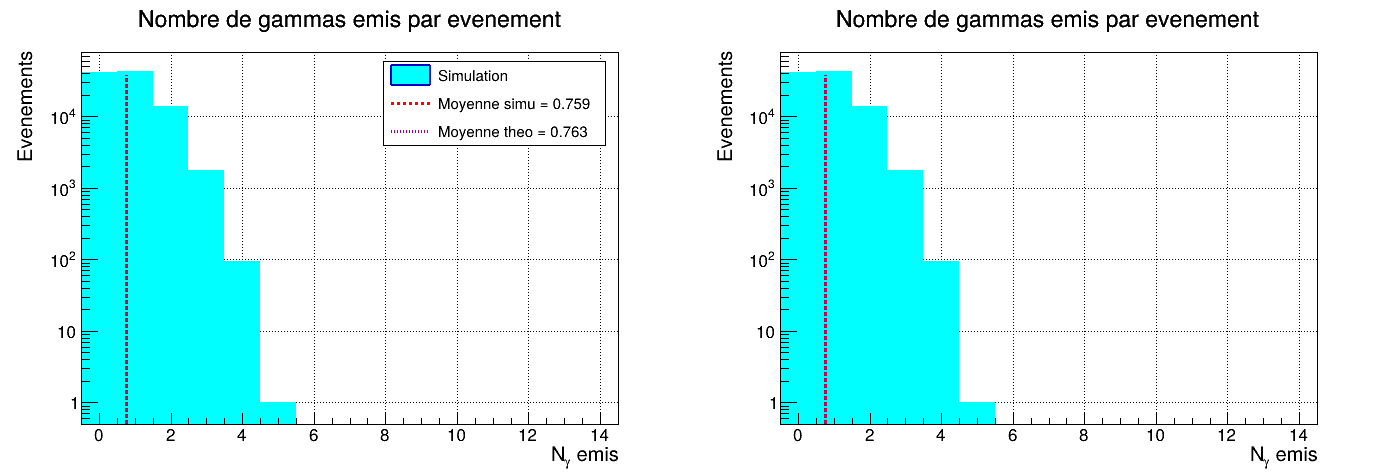
\includegraphics[width=0.95\textwidth]{emission_1_gamma_per_event.png}
    \caption{Distribution du nombre de gammas émis par événement. Gauche : échelle logarithmique avec lignes de moyenne. Droite : même distribution permettant de visualiser les événements à haute multiplicité.}
    \label{fig:gamma_per_event}
\end{figure}

\paragraph{Observations principales :}
\begin{itemize}
    \item La distribution est dominée par les événements à multiplicité 0 et 1, représentant chacun environ 42\% des désintégrations.
    \item La moyenne simulée est $\langle N_\gamma \rangle_{\text{simu}} = 0.759$, en excellent accord avec la valeur théorique $\langle N_\gamma \rangle_{\text{théo}} = 0.763$ (écart relatif $< 0.5\%$).
    \item Les événements à multiplicité $\geq 4$ sont rares ($< 0.1\%$), avec un maximum observé de 5 gammas.
    \item La distribution suit approximativement une loi de Poisson tronquée, caractéristique des processus de désexcitation nucléaire.
\end{itemize}

%==============================================================================
\section{Distribution des gammas par raie}
%==============================================================================

La figure~\ref{fig:gamma_per_line} montre la répartition des photons émis selon les 12 raies X et $\gamma$ de l'Am-241.

\begin{figure}[htbp]
    \centering
    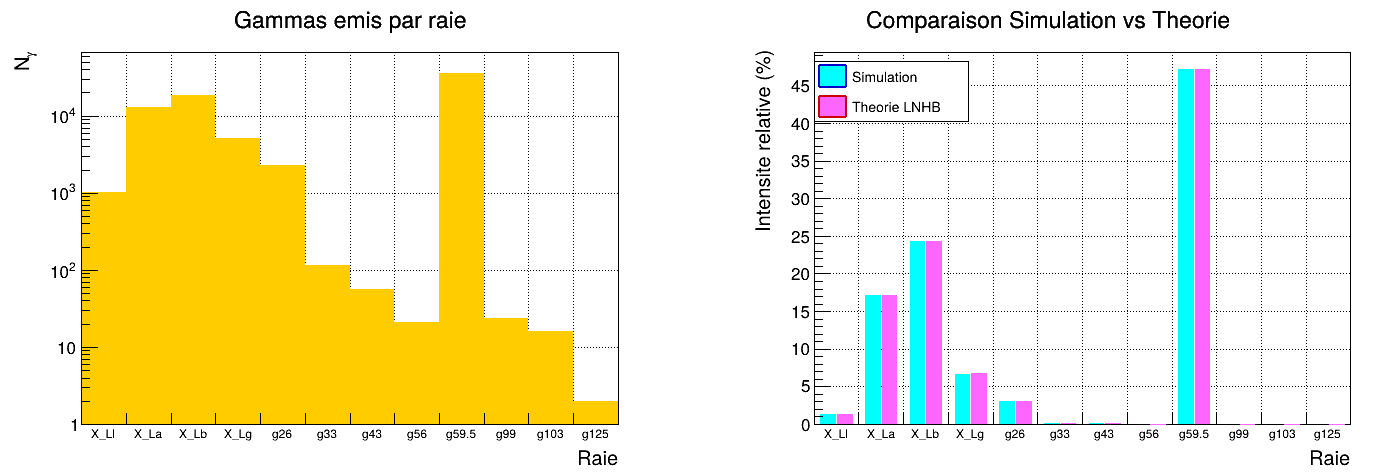
\includegraphics[width=0.95\textwidth]{emission_2_gamma_per_line.png}
    \caption{Gauche : nombre de gammas émis par raie (échelle log). Droite : comparaison des intensités relatives simulation/théorie LNHB.}
    \label{fig:gamma_per_line}
\end{figure}

\paragraph{Observations principales :}
\begin{itemize}
    \item La raie $\gamma$ principale à \SI{59.5}{keV} domine l'émission avec $\sim 47\%$ des photons.
    \item Les raies X-L du neptunium (X$_{\text{L}\alpha}$ à \SI{13.9}{keV}, X$_{\text{L}\beta}$ à \SI{17.0}{keV}) représentent ensemble $\sim 41\%$ de l'émission.
    \item L'accord simulation/théorie LNHB est excellent pour toutes les raies, validant l'implémentation du générateur primaire.
    \item Les raies de haute énergie ($\gamma_{99}$, $\gamma_{103}$, $\gamma_{125}$) ont des intensités très faibles ($< 0.05\%$).
\end{itemize}

\begin{table}[htbp]
    \centering
    \caption{Raies principales de l'Am-241 et leurs intensités.}
    \label{tab:raies}
    \begin{tabular}{llcc}
        \toprule
        Raie & Énergie (keV) & Intensité simu (\%) & Intensité théo (\%) \\
        \midrule
        $\gamma_{59.5}$ & 59.54 & 47.1 & 47.2 \\
        X$_{\text{L}\beta}$ & 17.0 & 24.4 & 24.3 \\
        X$_{\text{L}\alpha}$ & 13.9 & 17.1 & 17.1 \\
        X$_{\text{L}\gamma}$ & 20.8 & 6.7 & 6.8 \\
        $\gamma_{26}$ & 26.3 & 3.0 & 3.0 \\
        \bottomrule
    \end{tabular}
\end{table}

%==============================================================================
\section{Gammas primaires atteignant l'eau}
%==============================================================================

La figure~\ref{fig:gamma_water} présente la distribution des photons qui atteignent effectivement la cible d'eau après traversée de l'air.

\begin{figure}[htbp]
    \centering
    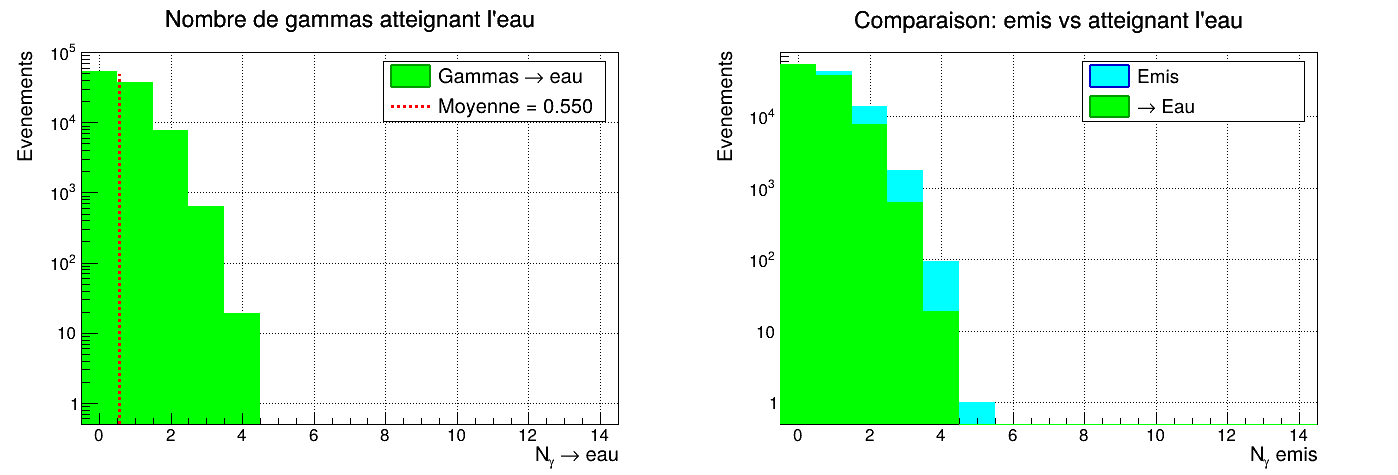
\includegraphics[width=0.95\textwidth]{emission_3_gamma_reaching_water.png}
    \caption{Gauche : distribution des gammas atteignant l'eau. Droite : comparaison avec les gammas émis.}
    \label{fig:gamma_water}
\end{figure}

\paragraph{Observations principales :}
\begin{itemize}
    \item La moyenne de gammas atteignant l'eau est $\langle N_{\gamma \to \text{eau}} \rangle = 0.550$ par événement.
    \item Le taux de transmission global est de $72.5\%$ ($0.550/0.759$).
    \item La comparaison des deux distributions (panneau droit) montre clairement les pertes : la distribution ``$\to$ Eau'' est systématiquement en dessous de la distribution ``Émis''.
    \item Les pertes sont principalement dues à l'acceptance géométrique (cône d'émission vs angle solide de la cible).
\end{itemize}

%==============================================================================
\section{Matrice Raie $\times$ Multiplicité}
%==============================================================================

La figure~\ref{fig:matrix_2D} présente l'histogramme 2D corrélant la raie émise avec la multiplicité totale de l'événement.

\begin{figure}[htbp]
    \centering
    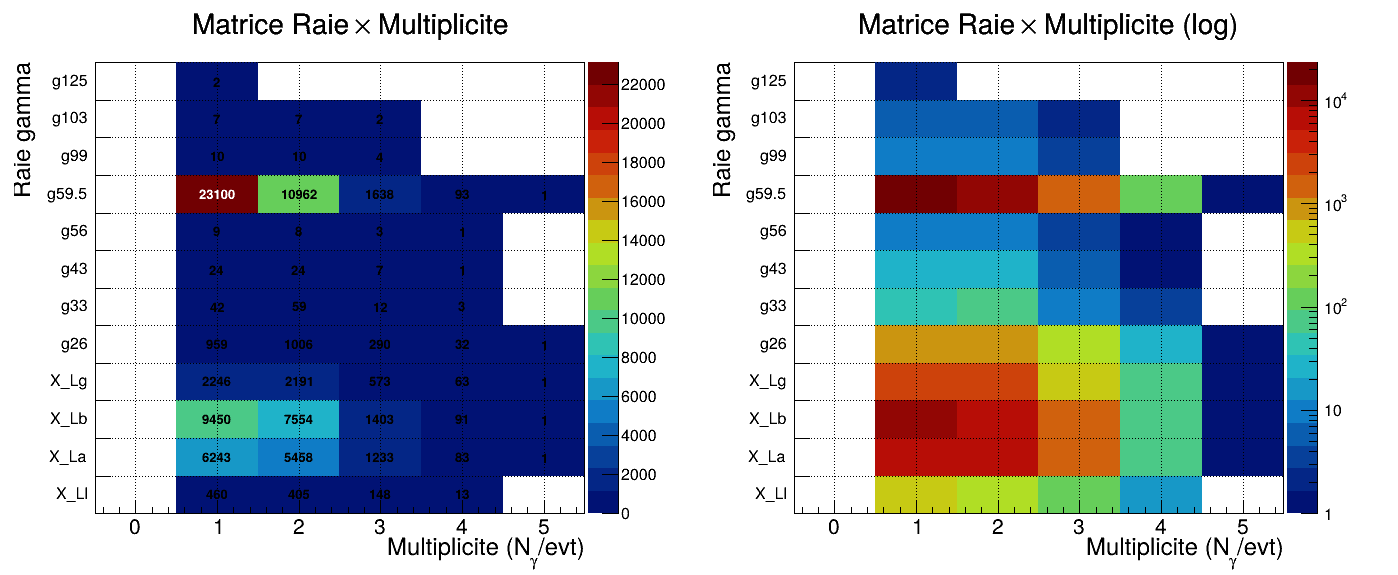
\includegraphics[width=0.95\textwidth]{emission_4_2D_line_vs_multiplicity.png}
    \caption{Matrice raie $\times$ multiplicité. Gauche : échelle linéaire avec valeurs. Droite : échelle logarithmique.}
    \label{fig:matrix_2D}
\end{figure}

\paragraph{Observations principales :}
\begin{itemize}
    \item À multiplicité 1, la raie $\gamma_{59.5}$ domine avec 23\,100 occurrences, suivie des raies X$_{\text{L}\beta}$ (9\,450) et X$_{\text{L}\alpha}$ (6\,243).
    \item À multiplicité 2, la raie $\gamma_{59.5}$ reste dominante (10\,962), souvent en coïncidence avec une raie X.
    \item Les raies de faible intensité ($\gamma_{99}$, $\gamma_{103}$, $\gamma_{125}$) n'apparaissent qu'aux faibles multiplicités.
    \item La colonne multiplicité 0 est vide par construction (pas de gamma $\Rightarrow$ pas de raie).
    \item L'échelle logarithmique (droite) révèle les corrélations pour les raies rares.
\end{itemize}

%==============================================================================
\section{Gammas perdus dans l'air}
%==============================================================================

La figure~\ref{fig:gamma_lost} analyse les photons qui n'atteignent pas la cible d'eau.

\begin{figure}[htbp]
    \centering
    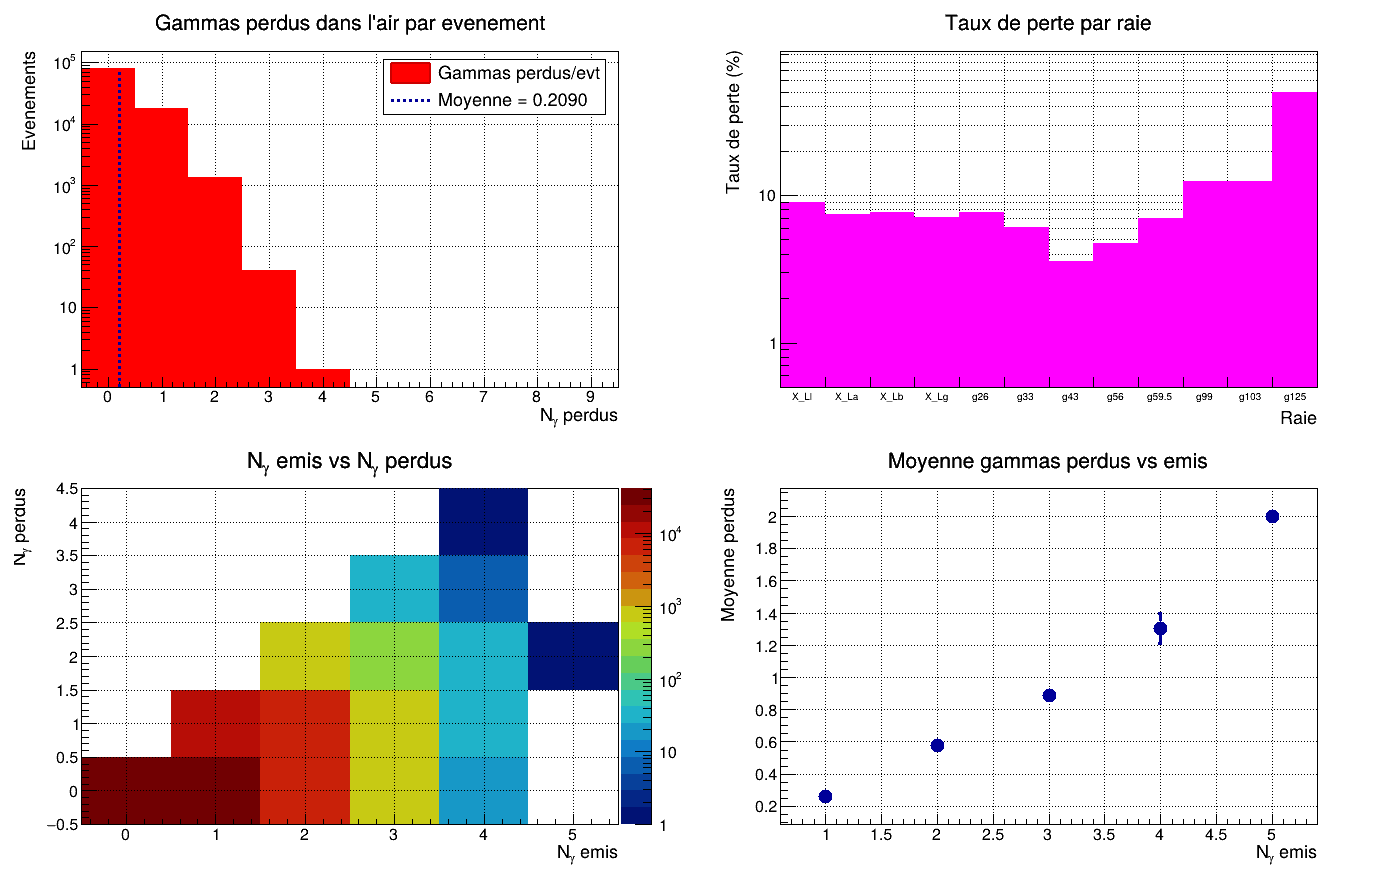
\includegraphics[width=0.95\textwidth]{emission_5_gamma_lost_in_air.png}
    \caption{Analyse des gammas perdus dans l'air. Haut gauche : distribution par événement. Haut droit : taux de perte par raie. Bas gauche : corrélation émis/perdus. Bas droit : moyenne conditionnelle.}
    \label{fig:gamma_lost}
\end{figure}

\paragraph{Observations principales :}
\begin{itemize}
    \item La grande majorité des événements ($\sim 95\%$) ne perdent aucun gamma dans l'air.
    \item La moyenne de gammas perdus est $\langle N_{\text{perdu}} \rangle = 0.209$ par événement.
    \item Le taux de perte par raie (haut droit) montre une tendance surprenante : les raies de haute énergie ($\gamma_{99}$, $\gamma_{103}$, $\gamma_{125}$) présentent des taux de perte plus élevés (10--50\%). Ceci est dû à la faible statistique de ces raies plutôt qu'à un effet physique.
    \item Les raies X et $\gamma_{59.5}$ ont des taux de perte homogènes autour de 7--9\%.
    \item La corrélation $N_{\text{émis}}$ vs $N_{\text{perdu}}$ (bas gauche) montre une relation quasi-linéaire.
    \item La moyenne conditionnelle (bas droit) confirme que le nombre moyen de gammas perdus croît linéairement avec le nombre émis, avec une pente $\approx 0.27$ correspondant au taux de perte géométrique.
\end{itemize}

%==============================================================================
\section{Conclusions}
%==============================================================================

Cette analyse de la statistique d'émission de la source Am-241 permet de conclure :

\begin{enumerate}
    \item \textbf{Validation du générateur} : L'excellent accord entre les intensités simulées et théoriques (LNHB) valide l'implémentation des 12 raies X/$\gamma$ dans le générateur primaire Geant4.
    
    \item \textbf{Multiplicité d'émission} : La moyenne de $0.759$ gamma/désintégration est conforme à la théorie. La distribution est dominée par les événements à 0 ou 1 photon.
    
    \item \textbf{Efficacité de transport} : $72.5\%$ des photons émis atteignent la cible d'eau, les pertes étant principalement géométriques (angle solide).
    
    \item \textbf{Raies dominantes} : La raie $\gamma$ à \SI{59.5}{keV} et les raies X-L du Np constituent $\sim 95\%$ de l'émission et dominent le dépôt de dose dans l'eau.
    
    \item \textbf{Pertes dans l'air} : Le taux de perte moyen de $\sim 7\%$ est cohérent avec l'acceptance géométrique du dispositif.
\end{enumerate}

\end{document}
